
\documentclass[10pt,a4paper]{article}
\usepackage[utf8]{inputenc}
\usepackage[french]{babel}
\usepackage[left=2cm,right=2cm,top=2cm,bottom=2cm]{geometry}
\usepackage{hyperref}
\usepackage{graphicx}

%opening
\title{TP2-Covid-19}
\author{Nicolas Vadkerti}
\usepackage{listings} % Required for inserting code snippets
\usepackage[usenames,dvipsnames]{color} % Required for specifying custom colors and referring to colors by name

\definecolor{DarkGreen}{rgb}{0.0,0.4,0.0} % Comment color
\definecolor{highlight}{RGB}{255,251,204} % Code highlight color

\lstdefinestyle{Style1}{ % Define a style for your code snippet, multiple definitions can be made if, for example, you wish to insert multiple code snippets using different programming languages into one document
language=Perl, % Detects keywords, comments, strings, functions, etc for the language specified
backgroundcolor=\color{highlight}, % Set the background color for the snippet - useful for highlighting
basicstyle=\footnotesize\ttfamily, % The default font size and style of the code
breakatwhitespace=false, % If true, only allows line breaks at white space
breaklines=true, % Automatic line breaking (prevents code from protruding outside the box)
captionpos=b, % Sets the caption position: b for bottom; t for top
commentstyle=\usefont{T1}{pcr}{m}{sl}\color{DarkGreen}, % Style of comments within the code - dark green courier font
deletekeywords={}, % If you want to delete any keywords from the current language separate them by commas
%escapeinside={\%}, % This allows you to escape to LaTeX using the character in the bracket
firstnumber=1, % Line numbers begin at line 1
frame=single, % Frame around the code box, value can be: none, leftline, topline, bottomline, lines, single, shadowbox
frameround=tttt, % Rounds the corners of the frame for the top left, top right, bottom left and bottom right positions
keywordstyle=\color{Blue}\bf, % Functions are bold and blue
morekeywords={}, % Add any functions no included by default here separated by commas
numbers=left, % Location of line numbers, can take the values of: none, left, right
numbersep=10pt, % Distance of line numbers from the code box
numberstyle=\tiny\color{Gray}, % Style used for line numbers
rulecolor=\color{black}, % Frame border color
showstringspaces=false, % Don't put marks in string spaces
showtabs=false, % Display tabs in the code as lines
stepnumber=5, % The step distance between line numbers, i.e. how often will lines be numbered
stringstyle=\color{Purple}, % Strings are purple
tabsize=2
}

\newcommand{\insertcode}[2]{\begin{itemize}\item[]\lstinputlisting[caption=#2,label=#1,style=Style1]{#1}\end{itemize}} 


% \insertcode{"Scripts/example.pl"}{Nena would be proud.} 



%  \begin{figure}[h!]
% \centering
% \includegraphics[scale=0.20]{image/2.jpg}
% \caption{Connection }
% \label{fig:net }
% \end{figure}


\begin{document}

\maketitle


\url{https://github.com/SlaynPool/CR_INP2/}

\section{Introduction}
La période que nous vivons actuellement est caractérisée par une pandémie de Coronavirus Covid-19. Ce virus est particulièrement dangereux pour les personnes de plus de 70 ans. Le contrôle régulier de leur température corporelle est très important afin de prévoir une hospitalisation dès la détection des premiers signes de fièvre afin d’éviter des complications. On se propose d’utiliser des objets connectés afin d’aider au suivi des températures de personnes à risque et d’effectuer des actions en cas de détection de fièvre.
\section{Fonctionnement désiré}
\subsection{Réseaux de collecte de données}
Notre objet doit avoir plusieurs caractéristiques essentiels, pour à la fois son bon fonctionnement, et la bonne utilisation par le patient. En effet, la partie informatique visible par le patient doit etre une interface simple pour que l'objet ce connecte au reseau wifi. De là, l'objet devra etre capable de communiquer avec un serveur qui sera chargé de récolter les données et le retransmettre au médecin traitant.\\ 
En terme d'infrastructure, nous devons garder en tête deux points fondamentale. Nos données sont vitales pour le patient donc il ne faut pas que nos paquets soit perdu sur le reseaux, et que l'information disparaisse, au risque de ne pas alerté le medecin et donc de mettre la vie du patient en danger. De plus, on doit pas oublier que les données que nous produisons sont soumis au secret médical et donc a des règles très strictes de stockages et de retention.\\
Pour le premier point, nous devrons obligatoirement utiliser des protocoles réseaux avec aquitements notaments via l'utilisation de TCP. On s'assura ainsi que les données seront émis et arriverons au niveau de tous les elements de l'infrastructure concernés. \\
Pour le second, nous devrons bien penser que les protocles et solutions de stockages devrons supporté des solutions de chiffrements pour que les données en notre possesions soit en ``sécurité''. Pour la partie réseaux, en pense evidements à SSL, implementé  sur STM32.
Pour ce qui est du protocole reseaux pour transmettre les data, on pourra utiliser MQTT. 
Pour Finir, pour ce qui est de la BDD, comme nous voulons stocker des data serialisée en focntion du Temps, nous utiliserons InfluxDB qui ce prête très bien à se genre d'application. InfluxDB supporte le chiffrements donc nous repondons parfaitement à la demande. Pour relier MQTT, et InfluxDB, nous utiliserons un agent type Telegraf pour remplir la BDD. 


\subsection{Décrire le protocole utilisé pour la collecte des données et indiquer les informations qui transitent.}
Un fois que la mesure sera effectué, les donnés emis grâce qu protocole MQTT à notre BDD pourra resembler à ceci : 
\begin{itemize}
 \item ID du Patient
 \item Date/heure de la mesure
 \item Mesure de temperature
\end{itemize}
Il suffira d'emetre sur le topic Mesure pour que le serveur récupère l'information. 
\subsection{ Ecrire un programme pour l’ESP32 permettant de répondre au fonctionnement demandé. On pourra s’inspirer du TP déjà réalisé permettant de mesurer la température ambiante }
Je n'implementerai pas la partie sécurité de l'objet, car cela nessecite l'infrastructure réseaux, ainsi que généré des clés Privé/Publique pour implementer SLL.

De plus, on suppose que nous avons une application graphique qui permettra à l'utilisateur de rentrée la configuration Wifi de son domicile et ainsi uploader le code sur l'objet avec la bonne configuration.

\insertcode{code/1.ino}{Premiere Implementation}

On suppose donc que l'objet dispose d'un bouton sur le pin 18 pour déclencher la mesure de temperature grâce au capteur DHT sur le pin 23. Dès que la mesure est éffectue les données sont emis sur grâce aux brokers MQTT sur le topic Temperature.



\subsection{Dans le but de se rapprocher le plus possible de la réalisation d’un objet réel, faire une recherche sur internet pour identifier un thermomètre médical pouvant s’interfacer avec notre plateforme ESP32 et modifier votre programme pour utiliser ce nouveau capteur. }



\subsection{Proposer une façon d’organiser votre base de données pour enregistrer les données provenant d’un grand nombre de plateformes ESP32}

On peut penser notre base de donnée comme ceci:\\ 
time  --    Patient     --  Mesure


Ainsi on pourra viens des requetes SQL simple faire des moyennes et suivre l'evolution dans le temps de la temperature du patient. 

\newpage
\section{Indication locale de la température }

\begin{figure}[h!]
\centering
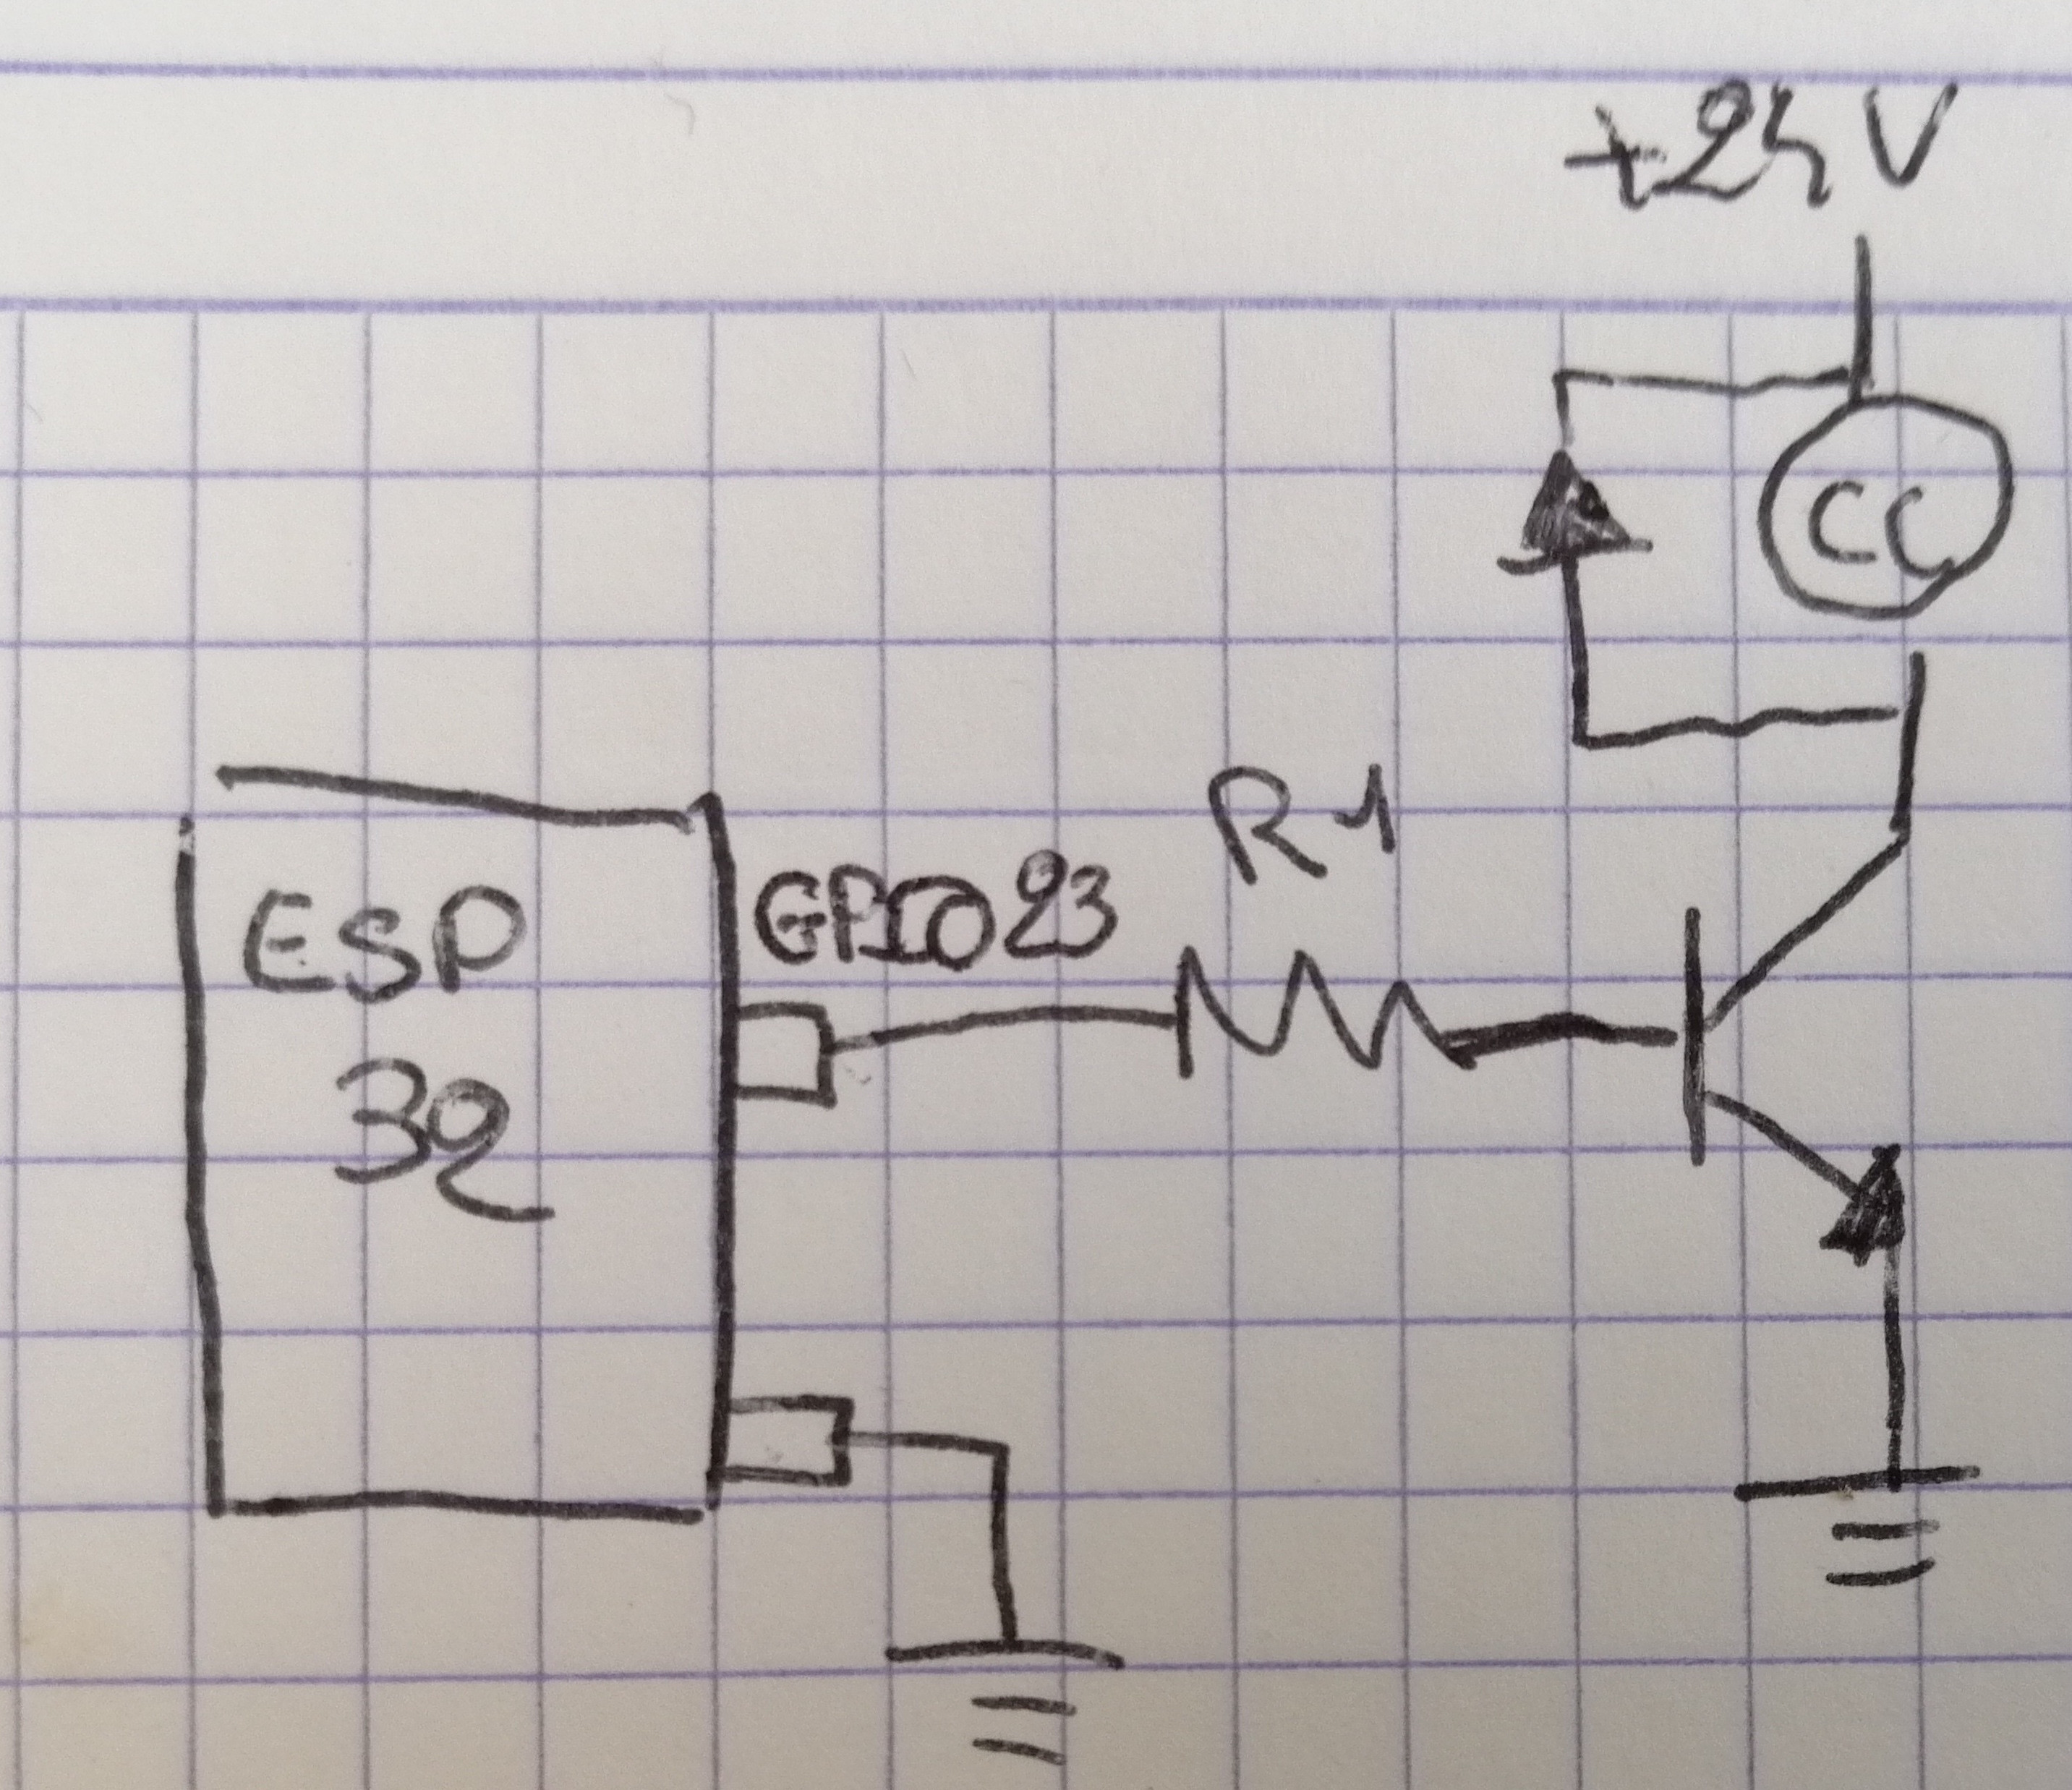
\includegraphics[scale=0.1]{image/1.jpg}
\caption{Connection }
\label{fig:net }
\end{figure}
\newpage
Nous modifions donc notre code en fonction.
\insertcode{code/2.ino}{code}\newpage

 
\section{Alerte d’une équipe de soins en cas de nécessité}
L'idée est simple, il suffirait d'avoir un esp32 connecter à un haut-Parleur et un ecran LCD. Notre systeme serait 
subscriber d'un topic /URGENCE sur lequel, notre code coté serveur, surveillerai toute les données qu'il recoit, et evalue si la situation est critique, et ainsi publirai sur le topic les urgences. Le message contiendrai l'addresse du patient, la fievre relevé. L.'objet pourrai alors afficher sur l'ecran LCD l'adresse du patient ainsi que généré un signal sonore pour prévenir l'equipe. A noter que cette objet pourrai largement etre remplacé par une application pour smartphone, car elle serait moins couteuse et plus simple d'utilisation.
\end{document}

